% ****** Start of file aipsamp.tex ******
%
%   This file is part of the AIP files in the AIP distribution for REVTeX 4.
%   Version 4.1 of REVTeX, October 2009
%
%   Copyright (c) 2009 American Institute of Physics.
%
%   See the AIP README file for restrictions and more information.
%
% TeX'ing this file requires that you have AMS-LaTeX 2.0 installed
% as well as the rest of the prerequisites for REVTeX 4.1
%
% It also requires running BibTeX. The commands are as follows:
%
%  1)  latex  aipsamp
%  2)  bibtex aipsamp
%  3)  latex  aipsamp
%  4)  latex  aipsamp
%
% Use this file as a source of example code for your aip document.
% Use the file aiptemplate.tex as a template for your document.
\documentclass[%
 aip,
 jmp,%
 amsmath,amssymb,
%preprint,%
 reprint,%
%author-year,%
%author-numerical,%
]{revtex4-1}
\usepackage{textcomp}
\usepackage{graphicx}% Include figure files
\usepackage{dcolumn}% Align table columns on decimal point
\usepackage{bm}% bold math
%\usepackage[mathlines]{lineno}% Enable numbering of text and display math
%\linenumbers\relax % Commence numbering lines

\usepackage{enumerate}
\usepackage{color}
\usepackage{xcolor}
\usepackage{listings}
\usepackage{caption}
\DeclareCaptionFont{white}{\color{white}}
\DeclareCaptionFormat{listing}{\colorbox{gray}{\parbox{\textwidth}{#1#2#3}}}
\captionsetup[lstlisting]{format=listing,labelfont=white,textfont=white}
\usepackage{tikz}
\usetikzlibrary{automata,arrows,positioning}
\usepackage[parfill]{parskip} % new paragraph no ident
\usepackage{hyperref}

\begin{document}

\preprint{AIP/123-QED}

\title[Lexicon Scanning for Compiler, a Computer Construction assignment report]{Compiler: Lexicon Scanning\\
A Go Implementation}% Force line breaks with \\
%\thanks{Footnote to title of article.}

\author{Ersi Ni}\thanks{15204230}
 \email{ersi.ni@ucdconnect.ie}
 \affiliation{University College Dublin, School of Computer Science}


\date{\today}% It is always \today, today,
             %  but any date may be explicitly specified

\begin{abstract}
This Compiler implementation is the result of open specification of courseware assignments for module Compiler Construction COMP30330 at UCD CSI, that any programming language can be used as long as it implements the requirements. The Compiler is implemented after chronological order the requirements from the courseware were released.
\begin{enumerate}[$\cdot$]
	\item Trie based Symbol table data structure
	\item Lexer
\end{enumerate}
To aid the testing and implementation, these components were also introduced:
\begin{enumerate}[$\cdot$]
	\item helper utilities
	\item test and benchmarking code
\end{enumerate}
\end{abstract}

\keywords{lexicon scanning, compiler construction, golang}
\maketitle

\begin{quotation}
The main reason of choosing Go to write the compiler, especially the lexer was
concurrency support and syntax support for function pointers.   \footnote{C can do all
this too, minus the practicality of enormous concurrency housekeeping}

Rob Pike has given a splendid talk about writing template system using Go,
particularly the Lexical Scanning, \url{https://www.youtube.com/watch?v=HxaD_trXwRE}
that talk has planted deep root for my implementation.
\end{quotation}

\section{\label{sec:level1}Data Structures}



\subsection{\label{sec:level2}Trie based Symbol Table}

The Symbol table is a lookup table for known Symbols, or identifiers. To
construct this lookup table a prefix tree (Trie) data structure is used to
process the input string.

To process ASCII characters the Trie features a bounded tree with the bound
equals to 128, so that the look up process has a temporal complexity of $O(d)$,
with the $d$ representing the depth of the tree, also as known as the length of
the input string.

The Trie stores information about the character and their meaning along the
path from the root: whether it completes word to form an Identifier or not;
and if it does, return the index of the word in the Symbol table.

\subsubsection{\label{sec:level3}Notes and Caveats}
The requirement of the module asks for handling characters range within ASCII
table. However the notion of "characters" is ambiguous in data presentation
level: depending on encoding scheme the data input chooses to adopt, a
"unicode" labeled input text might have ambiguous code points scheme that
requires normalization before proceeding to text processing. Also because Go
source code is always in UTF-8, it just makes sense to normalize texts input
either automatically using helper text normalization routine or manually saved
in UTF-8 encoding.

Specifically, we want to eliminate all multi rune
characters in the input text because they mess with rune based processing and
they are not in the ASCII range anyway.
See \url{https://en.wikipedia.org/wiki/Unicode_equivalence}
for background technicalities of this mess.

\section{Lexer}


\subsection{State Machine with Function Pointer}

The iniatialized lexer will start running with inital state and keep updating
itself: the state function does whatever it's supposed to do within the state,
triggers transition upon fulfilled condition and return the next state as a
function pointer, which is to be re-assigned to the same lexer.state variable.

The routine halts if the state machine reaches an accepting state, meaning 
the next state is \textbf{nil}.

\newpage

\begin{widetext}
\centering
\begin{lstlisting}[label=state-transition,caption=State Machine Transition]
func (receiver *Lexer) Run() {
	for receiver.State = startState; receiver.State != nil; {
		receiver.State = receiver.State(receiver)
	}
}
\end{lstlisting}
\end{widetext}

\subsubsection{State Machine Diagram}%

\begin{widetext}
\centering
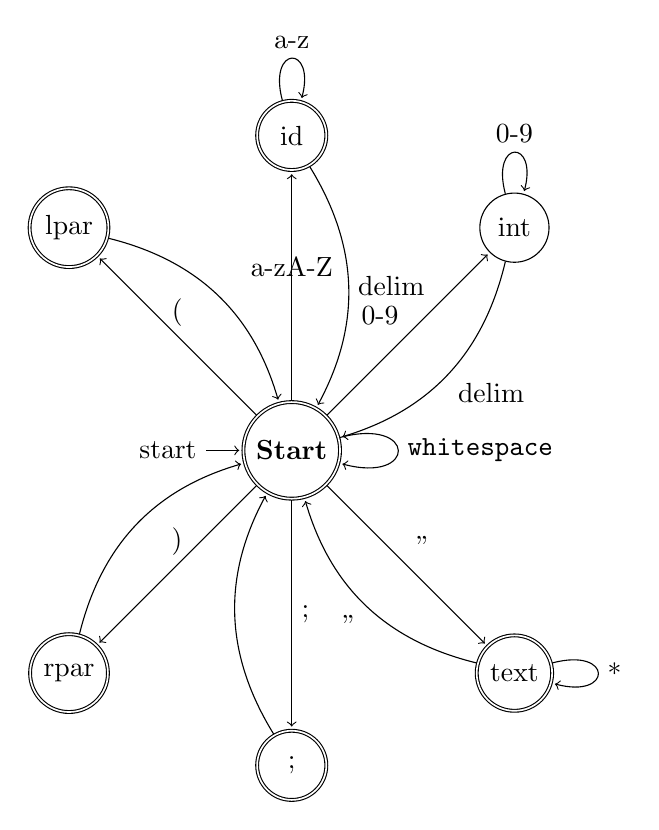
\begin{tikzpicture}[shorten >=1pt,node distance=4cm,on grid,auto] 
   \node[state,initial,accepting] (start)   {\textbf{Start}}; 
   \node[state] (int) [above right=of start] {int}; 
   \node[state,accepting] (text) [below right=of start] {text}; 
   \node[state,accepting](lpar) [above left=of start] {lpar};
   \node[state,accepting](id) [above=of start] {id};
   \node[state,accepting] (rpar) [below left=of start] {rpar};
   \node[state,accepting] (semicolon) [below=of start] {;};
   \path[->] 
   	(start) edge node {0-9} (int)
    		edge node[above] {a-zA-Z} (id)
		edge node[above]  {(} (lpar)
		edge node[above] {)} (rpar)
		edge node{;} (semicolon)
		edge node {"} (text)
		edge [loop right]node {$\mathtt{whitespace}$} ()
		
		(lpar) edge [bend left] node {} (start)
		(rpar) edge [bend left] node {} (start)		
		(semicolon) edge [bend left] node {} (start)
		(id) edge [loop above] node {a-z} ()
			edge [bend left] node {delim} (start)
		(int) edge [loop above] node {0-9} ()
			edge [bend left] node {delim} (start)			
		(text) edge [bend left] node {"} (start)
			edge [loop right] node {*} ()
    ;
\end{tikzpicture}
\end{widetext}

As shown in the diagram, {start}
is the main entry point, from there the immediate possible states, depending
on leading significant character, are {integer}, {identifier}, {keyword}
(static identifiers), {text} (string) and {singleToken}. Using function pointer
the {error} state doesn't need to be specified, instead the function pointer
will be set to nil, so the lexing will terminate.

There are details omitted in this diagram, mainly due to space constraints, such
as escaping with character {\large \texttildelow}, the definition of ``delim'' including
whitespace and state transition leading characters.

\subsubsection{Emit Tokens}

Upon successful lexing a token, the lexer emits this token to its message
channel, this channel can be consumed by a potential parser, a logging / print
mechanism or any interested party. One obvious feature of this implementation
is that the parsing and lexing can be run at the same time.

\subsubsection{Token Type}
Our Lexer deals with a language that has these token types:

\begin{table}[h]
\centering
\begin{tabular}{l|l}
$\mathbf{Type}$& Description \\
\hline
$\mathtt{id}$& identifiers \\
$\mathtt{int}$& integers \\
$\mathtt{lpar}$& left parenthesis \\
$\mathtt{rpar}$& right parenthesis \\
$\mathtt{semicolon}$& ;s \\
$\mathtt{string}$& strings \\
$\mathtt{error}$& errors
\end{tabular}
\end{table}

With whitespace characters deemed as natural delimiters, and at cases the
transition between $\mathtt{<id>}$ and $\mathtt{<int>}$ is also deemed as delimiter. The $\mathtt{<lpar>}$,
$\mathtt{<rpar>}$ and $\mathtt{<semicolon>}$ are both delimiter and tokens.
The error token will effectively terminate consumption from client.

\subsubsection{}



\end{document}
%
% ****** End of file aipsamp.tex ******
